%
% graphisch0.tex
%
% (c) 2020 Prof Dr Andreas Müller, Hochschule Rapperswil
%
\begin{figure}
\centering
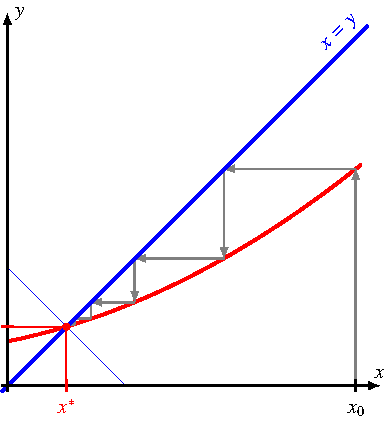
\includegraphics{chapters/10-arithmetik/figures/normal.pdf}
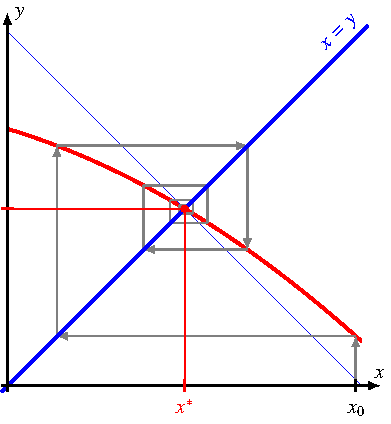
\includegraphics{chapters/10-arithmetik/figures/negativ.pdf}
\caption{Die Fixpunktiteration $x_{n+1}=f(x_n)$ konvergiert gegen
den Fixpunkt $x^*$ falls $|f'(x^*)|<1$ mit
mindestens linearer Konvergenzgeschwindigkeit.
\label{buch:figure:fixpunkt:normal}}
\end{figure}
